\chapter{Aplicação da programação linear na separação de pontos}

Na tarefa onde o obejtivo é a separação de dois ou mais conjuntos de pontos, sendo que cada conjunto representa um padrão, busca-se um método para que essa separação seja obtida com resultado ótimo. Cada conjunto é o resultado de um conjunto de pontos e cada ponto é é representado por um vetor de características.
Em \cite{Bennett92robustlinear} é proposto um modelo de programação linear capaz de um gerar um hiperplano de minimiza a soma dos pontos classificados de forma errada. Dessa forma o modelo é capaz de gerar um hiperplano separador para pontos linearmente separáveis e para conjutnos linearmente inseparáveis, o modelo gera o melhor hiperplano de forma que essa média calculada seja mínima. Na figura abaixo estão ilustrados os casos de dois conjuntos linearmente separáveis e dois conjuntos linearmente inseparáveis. COLOCAR FIGURA!!!
 
\begin{figure}
\centering
\subfigure[]{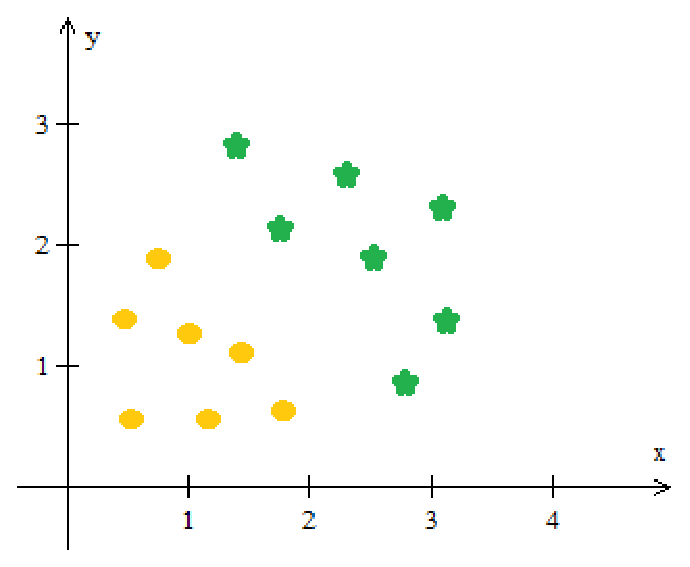
\includegraphics[scale=0.5]{graficos/linear_sepa}\label{fig1}}
\qquad
\subfigure[]{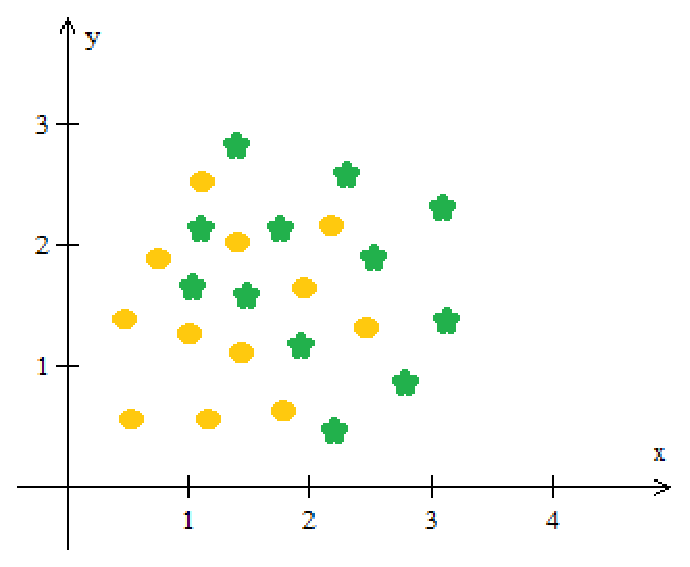
\includegraphics[scale=0.5]{graficos/linear_insepa}\label{fig2}}
\label{img:linear_sepa}
\caption{Em \ref{fig1} são apresentados dois conjuntos linearmente separáveis e em \ref{fig2} são apresentados dois conjuntos linearmente inseparáveis}
\end{figure}

\section{O modelo}
Considerando dois conjuntos, no espaço n-dimensional $ R^{n} $, sendo o conjunto A representado pela matriz m x n, e o conjunto B representado pela matriz k x n. Contextualizando, k e m são as quantidades de pontos em cada conjunto, e n é a quantidade de características. O modelo gera um hiperplano que separa os pontos dos dois conjuntos. De forma que os m pontos do conjunto A fiquem de um lado do hiperplano e os k pontos do conjunto B fiquem do outro lado do hiperplano. Na figura abaixo o modelo é apresentado. E a seguir é apresentado de forma mais detalhada.

COLOCAR MODELO!!!!

O modelo determina o hiperplano:
$$ x\omega = \gamma $$
Onde,  é $\omega$ o vetor normal ao hiperplano e $\gamma$ é um escalar. De forma que:
$$A\omega \geq e\gamma$$
e
$$B\omega \leq e\gamma$$
Onde e é um vetor de 1’s com dimensão m para o conjunto A e k para o conjunto B.
Para conjuntos linearmente separáveis torna-se fácil traçar um hiperplano separador, porém para conjuntos linearmente inseparáveis é necessária uma estratégia para que o hiperplano separador seja ótimo.
O modelo busca o melhor hiperplano, para isso gera dois hiperplanos limites somando 1 unidade a equação do hiperplano separador:
$$A\omega \geq e\gamma + e$$
e
$$B\omega \leq e\gamma - e$$
De forma que o hiperplano separador fica localizado exatamente entre esses dois hiperplanos limites.
Detalhando o modelo de acordo com \citeonline{Eberson10LPseparaPontos}, considerando x como um vetor em $ R^{n} $, definimos:

$1.\ \ (x_{i})_{+} = \max_{i=1,2,...,n}{\left \{x_{i},0  \right \}}$

$2.\ \ \left \| x \right \|_{1} = \sum_{i=1}^{n}\left | x_{i} \right |$

Podemos escrever o problema de minimização com norma da seguinte forma:

$$\min_{\omega ,\gamma }\frac{1}{m}\left \| \left ( -A\omega + e\gamma  + e \right )_{+} \right \|_{1} + \frac{1}{k}\left \| \left ( B\omega - e\gamma + e  \right )_{+} \right \|_{1}$$

Seja $g:R^{n} \mapsto R^{m} , h:R^{n} \mapsto R^{k}$ e S um subconjunto de $R^{n}$ . Os problemas abaixo possuem soluções idênticas:

$$\min_{x\in S}\left \| g(x)_{+} \right \|_{1} + \left \| h(x)_{+} \right \|_{1}$$


$$\min_{x\in S} e^{t}y + e^{t}z\\$$
$$ s.a.\left\{\begin{matrix}y\geq g(x)\\ \geq h(x)\\ y\geq 0, z\geq0\end{matrix}\right.$$
